\documentclass[a4paper]{report}
\usepackage{master}
\begin{document}

\author{Тузова Екатерина}
\title{Набор инструментов для поиска электронных книг в Интернете. Серверная часть, обеспечивающая верификацию, обновление данных и взаимодействие с клиентскими программами и пользователем.}

\maketitle
% подумать про заголовки
% TODO рассказать про автодополнения

\abstract{
Мотивацией для данного проекта послужило желание облегчить работу пользователей с электронными книгами. Ресурсы, которые сейчас есть в интеренете, позволяют пользователю последовательно сначала находить нужную книгу, затем самостоятельно скачивать и искать программу, которая может работать с файлом в заданном формате.

Основная идея проекта -- избавить пользователя от лишних и трудоемких действий, оставив ему самую приятную часть -- непосредственно чтение книги. Таким образом, проект призван объединить все стадии подготовки к чтению(поиск, скачивание, открытие файла) в одну. }

\newpage
\tableofcontents
\newpage

\section{Введение}
В последние годы влияние Интернета на жизнь человека становится все сильнее. Это обусловлено тем, что Интернет предоставляет гораздо больше удобства и возможностей для доступа к информации. Не оказалась в стороне от Интернета и такая важная часть работы и досуга, как чтение книг.

Двадцать лет назад для того, чтобы найти книгу человек шел в библиотеку или в книжный магазин. Если он искал определённую книгу -- достаточно было назвать фамилию автора и название книги, а порой даже одного названия было достаточно. Если же выбор книги ещё не был сделан, всегда можно было получить помощь от сотрудника магазина или библиотеки. Сегодня ситуация с библиотеками и книжными магазинами изменилась несильно, но наравне с бумажными книгами появилась возможность читать книги в электронном виде. 

Большое количество книг оцифровано и хранится в сети Интернет, многие из них находятся в свободном доступе. С одной стороны, это должно упрощать процесс получения книг, \tk теперь они стали доступны из любого места, где есть возможность выхода в Интернет. С другой стороны, перед пользователем встает новые проблемы. Во-первых, теперь ему необходимо самому искать книгу в сети, где количество информации растет с каждым днем. Во-вторых, после того, как он нашел нужную книгу -- ее нужно скачать, а затем найти программу, которая позволяет читать файл в найденном формате. 

%TODO 
На настоящий момент в Интернете существует множество электронных библиотек, поиск по которым весьма затруднен из-за того, что не существует системы, которая могла бы объединить всю информацию с этих библиотек. Следовательно, пользователям приходится либо искать в каждой из электронных библиотек в отдельности, либо пользоваться существующими поисковыми системами. Есть еще одна проблема, связанная с наличием большого количества электронных библиотек. Она состоит в том, что единый формат для предоставления информации о книгах появился только недавно, поэтому каждая библиотека предоставляет свой формат.

У существующих поисковых систем, в свою очередь,  есть одна очень важная особенность -- они обладают ограниченными возможностями в проведении специализированного поиска в сети. Поэтому в результате поиска пользователь получает всю информацию, которая соответствует поисковому запросу и дальше уже начинается работа самого пользователя над тем, чтобы эту информацию профильтровать и извлечь оттуда именно то, что ему нужно. 

Таким образом, выявляются две важные проблемы, затрудняющие поиск книг. Первая проблема -- различные библиотеки имеют разные интерфейсы, вторая -- существует множество форматов, в которых может быть представлена электронная книга. 

В данной работе была разработана система, упрощающая задачу поиска, чтения и управления книгами. 


\section{Обзор существующих решений}

Все эти проблемы не новы и попытки решить эти проблемы уже предпринимались.

Например, широко известная поисковая система Google предоставляет свой сервис для поиска электронных книг -- Google books (\url{http://books.google.com}). Этот сервис выполняет полнотекстовый поиск по книгам, которые Google сканирует и сохраняет в своей базе данных. В качестве результатов поиска выдается большое количество информации о самой книге, о различных изданиях этой книги и ссылки на ресурсы, где пользователь может приобрести книгу. Благодаря полнотекстовому поиску  по содержанию, есть возможность найти книгу, имея сильно ограниченное количество информации о ней. Этот сервис не решает ни проблему унифицированного доступа к информации о книгах, ни проблему различных форматов книг.

Сайт \url{http://ebdb.ru}(electronics books data base)  -- это поисковая система, которая обходит интернет и сохраняет у себя ссылки на те страницы сторонних ресурсов, которые содержат ссылки на книги. В результате поиска выдается список ссылок на страницы, содержащие книги. Для того, чтобы получить книгу пользователь должен перейти по ссылке, и, возможно, зарегистрироваться на ресурсе. Это решает проблему поиска книг, находящихся в свободном доступе, но остаются другие задачи, которые пользователь вынужден выполнять самостоятельно (скачивание книг и поиск подходящей программы для просмотра). Эта поисковая система тоже не решает проблемы унифицированного доступа и проблему различных форматов книг.

Есть большие системы, решающие проблему унифицированного доступа и различных форматов книг, а именно, Amazon Kindle, Sony Reader и подобные. 
Это программно-аппаратные платформы для чтения электронных книг. Они предоставляют устройство, которое имеет доступ к определенному хранилищу. Пользователь может подключить свое устройство к Интернету, найти нужную книгу в этом хранилище и купить ее. Дальше устройство само скачает книгу и откроет ее.
Из минусов у таких систем то, что эти системы платные и зависимые от устройства. Количество доступных книг -- ограничено теми книгами, которые хранят/продают хранилища, к которым они подключаются. Но это не единственные минусы таких систем. Так, к примеру, у Amazon Kindle за каждый загруженный текст (вне зависимости от источника загрузки) требуется заплатить компании Amazon от 10 центов. Еще Amazon контролирует информацию, содержащуюся на устройствах, находящихся у пользователей и по своему усмотрению удаляет её (в том числе книги, приобретённые непосредственно у Amazon).

Существует открытая технология, решающая проблему унифицированного доступа  -- OPDS (Open Publication Distribution System).
OPDS -- это новый активно развивающийся стандарт, который построен на базе расширяемого языка разметки Atom. Этот стандарт был специально разработан для предоставления информации об электронных документах. В нем учтены особенности такого рода информации (наличие аннотации, автора, изображения обложки и пр.).
Основная идея существования такого стандарта в том, что если многие сайты будут распостранять свою информацию о книгах в таком формате, то клиентские программы могут работать с ними единообразно (см. \picref{fig:scheme}). Несмотря на то, что стандарт появился недавно, уже существуют сайты и клиетские программы, использующие этот протокол. 

\begin{figure}
\centering
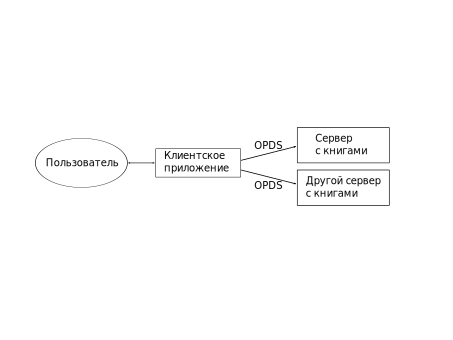
\includegraphics[width=.5\textwidth]{scheme}
\caption{Схема взаимодействия с использованием формата OPDS}\label{fig:scheme}
\end{figure}

Одим из самых крупных сайтов, предоставляющих информацию по протоколу OPDS, является BookServer (\url{http://bookserver.archive.org}).
Этот некоммерческий проект является частью проекта Internet Archive (\url{http://archive.org}) и является универсальной и открытой системой распостранения электронных книг. BookServer это архитектура, объединяющая различные форматы книг, конвертируя их, при необходимости, в нужный формат. Система обеспечивает каталогизацию книг, имеющихся в магазинах, библиотеках или в открытом доступе. Электронный текст можно прочитать на любом конечном устройстве, будь то нетбук, смартфон или специализированное устройство для чтения, наподобие Kindle. Хотя сайтом уже можно пользоваться, он еще находится на стадии разработки, с чем, вероятно, связано отсутствие расширенного поиска по книгам, фильтрации по языкам/жанрам. Так же, минусом этого проекта для русскоговорящих пользователей является невозможность поиска с использованием русских символов.

%TODO BEGIN
\section{Описание системы в целом}
Проект состоит из серверной и клиентской частей.

Серверная часть собирает в сети Интернет информацию об электронных книгах и представляет собранную информацию для обычных пользователей в виде web-интерфейса и для клиентских программ -- в формате OPDS.

Клиентская часть представляет собой программу для удобной работы с сервером, предоставляющим по запросам информацию в формате OPDS. Клиент должен работать как с "родным" сервером, так и с другими серверами, поддерживающими OPDS, например feedbooks.com.

Серверная часть проекта состоит из 3 подпроектов:
\begin{itemize}
	\item собственно web-сервер, включающий базу данных, поиск по ней, представление информации в web и opds форматах (python, django)
	\item сборщик информации в сети (crawler) (java)
	\item анализатор найденной информации, разбирающий информацию о книгах (java) 
\end{itemize}
Клиентских программ написано 2:
\begin{itemize}
	\item На С++ (с интерфейсом Qt)
	\item На Java 
\end{itemize}

Клиентская программа на Java более переносима, но для нее необходимо на девайсе иметь java-машину. В свою очердь программа на Qt не требует установки никаких дополнительных библиотек, работает быстрее, но переносимость ниже, чем у java.
		
\section{Описание компонентов системы и их взаимодействие}

% Может стоит вставить пару картинок

Пользователь устанавливает у себя на машине одну из клиентских программ. При поиске книги программа обращается к одному из серверов, поддерживающих протокол OPDS,(OpenSearch?). Сервер обрабатывает запрос, и возвращает данные в в нужном формате. 
% TODO STOP





\section{Постановка задачи}

Основой для данной работы послужили задачи поиска дополнительной информации, а так же верификация данных, их структурирование  и предоставление пользователю и клиентским программам.


\subsection{Верификация и обновление данных}

После того, как книги найдены и добавлены в базу данных требуется все время поддерживать ее в рабочем состоянии, обновлять имеющуюся инфомацию и производить поиск дополнительной.

Верификация нужна потому, что информация, поступающая от "поискового паука" (crawler) и анализатора (analyzer) зачастую бывает весьма сомнительного качества. Это происходит из-за того, что иногда "поисковый паук" находит книги, находящиеся на "сложных" страницах. С таких страниц анализатор либо не может извлечь информацию об авторе и названии книги, либо извлекает ее с ошибками. 

Если анализатор не может определить автора/название, то в базу добавляется только ссылка на файл. Позже необходимо извлечь максимум доступной информации либо из самого файла, если это возможно, либо из других источников.

Часто возникают ситуации, когда со страницы с найденной книгой возможно извлечь только информацию об авторе и названии книги. Сервер же ориентирован на предоставление информации о книгах в удобном для пользователя виде. Одним из таких способов является разбиение книг по таким каталогам, как различные языки и жанры. Для обеспечения лучшего разбиения по таким каталогам необходимо реализовать поиск дополнительной информации, такой как аннотация, теги и пр., для книг и авторов, которые уже находятся в базе.


Так же существует вероятность, что информация об авторе и названии книги извлечена со станицы с ошибками. В таком случае необходимо предоставить возможность администратору исправлять её достаточно простым способом, например, через web-интерфейс.


\subsection{Предоставление данных}

Сервер должен предоставлять информацию двумя способами -- в HTML виде для пользователей, желающих использовать web-browser, и по протоколу OPDS -- для клиентских программ. Предоставление данных должно быть удобным для пользователя. Должен присутствовать простой и расширенный поиск, а так же разделение данных по каталогам. Для предоставления информации необходимо описать логику отображения информации и способы ее отображения. Необходимо реализовать поддержку протокола OPDS, а также поддержку технологии OpenSearch.


\section{Задача верификации и обновления информации}

После того, как книги найдены и добавлены в базу данных требуется все время поддерживать ее в рабочем состоянии, обновлять имеющуюся инфомацию и производить поиск дополнительной. Возникают задачи верификации и обновления информации. Для решения задачи верификации -- реализован интерфейс администратора, для обновления и пополнения базы данных -- поиск информации на внешних ресурсах, классификация книг на основе аннотации, поиск информации внутри отдельной книги.

\subsection{Задача определения жанра книги}

На сервере хранится база данных, заполненная собранной в интернете информацией о книгах. В информацию о книге входят -- название, автор, описание, жанр и некоторые другие поля. Обязательными для книги являются название книги и автор (у каждой книги может быть указано больше одного автора). Для некоторых книг в найденной информации уже указан жанр, для других -- нет. Для более удобной навигации пользователя по базе, сервер предоставляет возможность различных выборок, в том числе по жанру, но для многих книг анализатор не может определить жанр, исходя из информации, находящейся на той странице, где была найдена книга. Для предоставления пользователю более полной информации реализовано определение жанра книги, исходя из её аннотации. 

Для реализации были использованы техники искусственного интеллекта, а именно машинного обучения. Машиное обучение -- это обширный подраздел искусственного интеллекта, изучающий методы построения алгоритмов, способных обучаться. В большинстве случаев это означает, что алгоритму подается на вход набор данных, а он выводит информацию о свойствах этих данных, причем так, что на основе выведенной информации способен делать предсказания о данных, которые может увидеть в будущем. Это возможно потому, что практически все неслучайные данные содержат какие-то закономерности (паттерны) и, выявив их, машина способна сделать обобщение. У машинного обучения есть свои слабости. Алгоритмы различаются по способности делать обобщения на основе больших наборов паттернов, и если некий паттерн никогда прежде не встречался, то возможна его ошибочная интерпретация. Природа алгоритмов машинного обучения такова, что они продолжают обучаться по мере поступления новой информации.

Для реализации определения жанра книги рассматривались многие возможности машинного обучения, а именно методы обучения с учителем, такие как Байесовский классификатор, деревья решений, нейронные сети, метод к-средних и пр. Классификатор, построенный на основе деревьев решений не поддерживает инкрементальное обучение, так жк дерево для больших наборов данных может оказаться слишком большим, что существенно замедлит процесс классификации. Нейронные сети поддерживают инкрементальное обучение, но являются своего рода "черным ящиком". В реальных сетях имеются сотни нейронов и тысячи синапсов, поэтому понять как сеть выбрала ответ невозможно, что делает невозможным более тонкую ручную настройку. Основным недостатком метода к-средних является то, что для прогнозирования ему требуются все данные, на которых производилось обучение. На это расходуется не толлько память, но и время -- для выработки каждого прогноза приходится сравнивать новый образец с каждым из имеющихся, чтобы найти ближайшие. 

В итоге проведенного анализа алгоритмов, для реализации был выбран Байесовский классификатор, \tk это наиболее подходящий классификатор для обучения и опрашивания на больших наборах данных. Даже если обучающий набор очень велик, обычно для каждого образца есть лишь небольшое количество признаков, а обучение и классификация сводятся к простым математическим операциям над вероятностями признаков. Важной особенностью такого классификатора является возможность инкрементного обучения, \te каждый новый предъявленный образец можно использовать для обновления вероятностей без использования старых обучающих данных. Поддержка инкрементного обучения важна, \tk это дает возможность классификатору обучаться на вновь поступающих в базу данных книгах. Классификатор должен обновляться быстро и без дополнительных запросов к базе данных о книгах, на которых был обучен. Ещё одно достоинство наивного Байесовского классификатора -- относительная простота интерпретации того, чему классификатор обучился. Это позволяет более точно настраивать полученный классификатор, изменяя вероятности для некоторых признаков.


 Для определения жанра книги создан классификатор, построенный на основе наивного байесовского классификатора. Наивный байесовский классификатор это простой вероятностный классификатор, основанный на применении Теоремы Байеса со строгими (наивными) предположениями о независимости. Для определения вероятности для всего документа был выбран метода Фишера. 
В отличие от наивной байесовсой фильтрации, когда для вычисления вероятности всего документа перемножаются вероятности отдельных признаков, по методу Фишера вычисляется вероятность отнесения к той или иной категории для каждого признака документа, после чего эти вероятности комбинируются и проверяется, насколько получившееся множество похоже на случайное.

В качестве входа классификатор принимает текст. Этот текст разбивается на слова. Каждое слово подвергается стеммингу. Стемминг -- это процесс нахождения основы слова для заданного исходного слова. Основа слова необязательно совпадает с морфологическим корнем слова. В итоговый вектор добавляются все слова и пары слов, встреченные в тексте.

В случае классификации книг в качестве текста были взяты название книги и ее аннотация. В том случае, если описание  еще не хранится базе данных происходит поиск на Amazone.

Таким образом во время классификации частично решается задача поиска дополнительной информации о книгах на внешних ресурсах.


\subsection{Поиск информации на внешних ресурсах}

Задача поиска дополнительной информации решается одновременно с решением других задач. Например, поиск аннотации для книг производится во время их классификации по жанрам.
В работе реализован поиск дополнительной информации на сайте Amazon (\url {http://amazon.com}) - поиск аннотации для книг, на сайте wikipedia (\url {http://en.wikipedia.org}) происходит поиск дополнительной информации для авторов(теги).

Для поиска информации о книгах на внешних ресурсах необходимо анализировать большие объемы HTML страниц, \tk пока не существует ресурсов, предоставляющих информацию о большом количестве книг в унифицированном формате. Для обработки страниц использовалась библиотека Beautiful Soup. Beautiful Soup -- это написанный на Python анализатор документов в форматах HTML и XML. Он спроектирован так, что способен работать с плохо написанными  веб-страницами. Одновременно с этим, библиотека предоставляет достаточно удобный интерфейс использования.

\subsection{Извлечение информации из форматов epub и fb2}

Для пополнения базы данных так же используется извлечение информации из книг в формате epub и fb2. В случае если анализатор не смог определить название полученной от поискового паука книги и ее автора, но найденный файл в фомате fb2 или epub, в базу данных добавляется ссылка на этот файл, но эта ссылка не привязывается ни к какой книге. Это делается, \tk из этих форматов можно извлечь нужную информацию. 

%TODO может быть xml схемы?
Electronic Publication (ePub) — открытый формат электронных версий книг. Формат позволяет издателям производить и распространять цифровую публикацию в одном файле, обеспечивая совместимость между программным и аппаратным обеспечением, необходимым для воспроизведения незашифрованных цифровых книг и других публикаций с плавающей вёрсткой.
Zip-архив контейнера ePub содержит тексты в форматах xHTML, HTML или PDF, описание издания в XML, рядом в папках — графика, включая векторную (SVG), и встроенные шрифты, таблицы стилей и \td 

FictionBook — формат представления электронных версий книг в вие XML-документов, где каждый элемент книги описывается своими тегами. Стандарт призван обеспечить совместимость с любыми устройствами и форматами. XML позволяет легко создавать документы, готовые к непосредственному использованию и программной обработке (конвертации, хранению, управлению) в любой среде. Документы содержат структурную разметку основных элементов текста, некоторое количество информации о книге, а также могут содержать вложения с двоичными файлами, в которых могут храниться иллюстрации или обложка.

Оба формата хранят информацию о книге в удобном для автоматической обработки формате. Оба формата имеют xsl-схему, с помощью которой происходит валидация документа и с помощью которой был написан парсер извлекающий нужную информацию.

\subsection{Реализация интерфейса администратора}
%TODO может надо про то, как он генерируется рассказать. А то как то сразу про настройку.

В Django есть встроенный интерфейс администратора. Это веб-интерфейс, доступный администраторам сайта, который предоставляет возможность добавления, редактирования и удаления содержимого сайта. Получая метаданные из описанных моделей, он предоставляет мощный интерфейс промышленного уровня, который может быть немедленно использован для наполнения сайта информацией.

Каждый тип обьектов в интерфейсе администратора обладает формой редактирования и списком обьектов. Список объектов отображает все доступные обьекты в базе данных, а форма редактирования позволяет добавлять, изменять и удалять конкретные записи. 
Разные типы полей имеют разное отображение (виджеты) -- например, поля даты/времени управляются через календарь, булево поле -- через чекбокс, текстовое поле -- обычное поле ввода. 
Автоматическая генерация интерфейса администратора удобна, но ввиду того, что это очень общая задача -- некоторые типы полей отображаются очень неудобно для редактирования. Интерфейс администратора предназначен для использования неквалифицированными пользователями и, следовательно, он должен быть самодостаточным.

\subsubsection{Как появляется интерфейс администратора}

Когда Django загружает схему URL из url.py  при старте сервера, выполняется функция admin.autodiscover(), которая добавиляется для активации интерфейса администрации. Эта функция проходит по элементам параметра INSTALLED\_ APPS и проверяет наличие файла admin.py в каждом установленом приложении. Если файл присутствует, выполняется его код. Внутри этого файла происходит регистрация моделей в интерфейсе администратора. %TODO пример

Простая настройка интерфейса администратора предоставляет немного возможностей - сделать поля необязательными, изменить метки полей, выбрать из ограниченного набора способ, которым будет отображаться поле.

Несмотря на всё это, административный интерфейс является всего навсего простым приложением Django, со своими собственными моделями, шаблонами, представлениями и схемой URL. Таким образом есть возможность настройки этого интерфейса для своего приложения.

\subsubsection{Задачи, которые не решает встроенный интерфейс}
\begin{itemize}
	\item Отображение полей многие-ко-многим.
	\item Поиск
	\item Проверка орфографии в TextArea
\end{itemize}

%\subsection{Решения}
Одной из главных проблем интерфейса администратора является ограниченный выбор способа отображения полей многие-ко-многим. В интерфейсе, предоставляемом Django -- для отображения таких полей есть несколько возможностей(виджетов):
\begin{itemize}
	\item Select -- список с возможностью множественного выбора.
	\item Filter horizontal/vertical -- два списка (horizontal/vertical определяет их относительное местоположение). Один из списков представляет собой список всех вожможных вариантов выбора, второй -- выбранные элементы.
	\item Raw\_ id -- представляет собой input-строку, с перечисленными в ней id выбранных элементов. Есть возможность добавлять элементы.
\end{itemize}
Первые два варианта -- загружают в список все возможные варианты выбора целиком. Для модели, содержащей большое количество связей типа многие-ко-многим этот вариант не подходит, \tk загружать весь список становится слишком долго. Хотя, надо заметить, что на небольшом количестве таких связей такое отображение выглядит очень удобно( В представленной базе данных это отображение используется для связей тег-книга). 
Третий вариант больше подходит для отображения большого количества связей, но у него есть один недостаток -- в текстовом поле отображаются только id элементов, связанных с данным. Очень маловероятно, что человеку (администратору) будет удобно оперировать в терминах id объектов.

Таким образом возникает задача создания удобного виджета для отображения авторов, связанных с конкретной книгой.
Было решено реализовать эту связь в формате нескольких checkbox'ов, с возможностью добавлять
новые.

\subsubsection{Реализация}

При создании интерфейса администратора для каждой модели в базе данных создаются классы ModelAdmin, которые предоставляют возможности настройки его работы для конкретной модели. При регистрации этой модели есть возможность указать форму, которая будет использоваться при отображении. При регистрации модели Book из базы данных была указана специально созданная форма для отображения -- BookForm. Далее для создания формы был написан класс, который наследуется от стандартного класса Django forms.ModelForm. Внутри созданной формы для каждого из полей модели можно специфицировать используемый виджет.

Для создания виджета, отображающего поле типа многие-ко-многим нужно указать способ отображения raw\_ id, тогда в темплейт будут передаваться идентификаторы элементов, связанных с данным. Далее нужно создать собственный виджет для отображения данных об авторе книги AuthorWidget. 

Для обеспечения нужного поведение класс AuthorWidget наследуется от стандартных классов Django CheckboxSelectMultiple и ManyToManyRawIdWidget. Класс CheckboxSelectMultiple предоставляет методы, помогающие сконструировать виджет. Класс ManyToManyRawIdWidget предоставляет методы, позволяющие сохранить информацию в базу данных. В полученном классе осталось определить метод create\_ content, который определяет содержимое виджета и переопределить метод render, который будет вызывать метод родительского класса CheckboxSelectMultiple, передавая ему нужные параметры. 

Внутри метода create\_ content, которому передаются идентификаторы отображаемых элементов происходит обращение к базе и по идентификатору определяются имена авторов. Затем используется метод render родительского класса, которому передаётся список пар (author\_ id, author\_ name). Этот метод генерирут представление поля в нужном формате.

После того, как информация правильно отображена на странице нужно научиться сохранять ее в базе данных. За сохранение  информации в базу данных отвечает форма BookForm, которая указана в классе ModelAdmin для модели Book. Для того, чтобы информация правильно сохранялась нужно переопределить метод save. В стандартном методе, который наследуется от родительского класса ModelForm используется метод cleaned\_ data. Этот метод извлекает информацию из форм. Затем в методе save происходит проверка -- изменилась ли эта информация и, если информация изменилась, происходит ее сохранение в базу данных. Метод cleaned\_ data извлекает из checkbox не только идентификатор элемента, а для сохранения поля в базу данных методу нужно передать идентификатор. Для этого в переопределенном методе save извлекается cleaned\_ data, затем из cleaned\_ data извлекается информация, связанная с виджетом, отображающим авторов. Из этой информации извлекаются идентификаторы элементов и сохраняются в изначальный словарь. Затем вызывается метод save родительского класса ModelAdmin, которому передается уже измнённый словарь значений cleaned\_ data. 

После того, как информация об авторах предоставляется в удобном виде и правильно сохраняется в базу данных необходимо предоставить пользователю интерфейса администратора возможность добавления авторов. 

Эту возможность было решено реализовать в виде открытия (по требованию) нового окошка со списком авторов с возможностью поиска по авторам. После того,как выбран определённый автор окошко закрывается, а в основном окне появляется CheckBox с именем автора. 

Для реализации этой возможности во многом используется Javascript. В интерфейсе администратора есть возможность подключать сторонний Javascript. Для этого в той форме, для отображения которой нужно использовать Javascript это явно указывается таким образом:

\begin{verbatim}
class AuthorForm(forms.ModelForm):
    class Media:
    	model = Author
        js = ('RelatedObjectsLookups.js',)

\end{verbatim}

Для начала в форму, отображающую авторов нужно добавить кнопку, после нажатия которой будет вызываться вспомогательное окошко. Это делается в методе render, который переопределен для AuthorWidget. Как было сказано выше в методе render вызывается метод, генерирующий содержание виджета, а затем вызывается метод родительского класса, который возвращает сам виджет. К нему добавляется ссылка, по щелчку на которой, вызывается Javascript. Интерфейс администратора предоставляет функцию javascript, которой нужно указать ссылку, которую нужно открыть в новом окне. Эта функция будет вызываться по щелчку. 

При выборе автора из списка вызывается функция dismissRelatedLookupPopup. Эту функцию нужно адаптировать к виджету, отображающему авторов. Функция должна находить по идентификатору на странице виджет, отображающий авторов и добавлять еще один checkbox с именем автора. Проблема состоит в том, что при вызове -- этой функции передаются только идентификаторы выбранных элементов. 

Чтобы изменить такое поведение нужно воспользоваться еще одной возможностью Django. Для автоматической генерации темплейтов для моделей в интерфейсе администратора используется вызов функции result\_ list. Внутри этой функции генерируется содержание темплейта, который будет вызван при открытии вспомогательного окошка. Чтобы передавать в Javascript нужные параметры необходимо переопределить эту функцию и явно внутри указать аккие параметры будут переданы Javascript'у.


\numlesschap{ Задача представления информации}

Информация, хранящаяся на сервере, предоставляется двумя способами -- в виде HTML для пользователей, желающих использовать web-browser, и по протоколу OPDS -- для клиентских программ. Фреймворк Django, использованный для реализации приложения, позволяет использовать очень высокий уровень абстракции.

Главной идеей в Django является разделение задач. Каждая задача выделена в отдельный файл:
% TODO Для каждого из пунктов вставить маленький кусочек кода
\begin{itemize}
	\item Файл models.py содержит описание таблицы базы данных, представленное в виде класса Python. Такой класс называется моделью. С помощью данного класса можно создавать, получать, обновлять и удалять записи в таблице базы данных, используя простой код на языке Python вместо использования повторяющихся SQL команд.
	\item Файл views.py содержит логику отображения страницы. В этом файле содержатся функции, которым передается URL запрос. Такие функции называются представлением.
	\item Файл urls.py определяет какое именно представление будет вызвано для URL, заданного в виде шаблона. 
	\item Так же есть файлы-шаблоны, которые описывают дизайн страницы. Эти файлы используют свой шаблонный язык.
\end{itemize}

 Объединённые вместе, эти компоненты приложения следуют шаблону Модель-Представление-Управление  (Model-View-Controller, MVC). MVC определяет способ разработки программного обеспечения при котором код для определения и доступа к данным (модель) отделён от логики приложения (управление), которая в свою очередь отделена от интерфейса пользователя (представление). В этой концепции термин «Модель» относится к логике доступа к данным; термин «Представление» относится к той части системы, которая определяет, что показать и как; а термин «Управление» относится к той части системы, которая определяет какое представление надо использовать, в зависимости от пользовательского ввода, по необходимости получая доступ к модели. 

Шаблон Django — это строка текста, которая предназначена для отделения представления документа от его данных. Шаблон определяет места подстановки и различные виды основной логики (шаблонные теги), которая управляет отображением документа. Обычно, шаблоны используются для создания HTML, но шаблоны Django также способны участвовать в генерации любого текстового формата.

Основное преимущество такого подхода заключается в свободе объединения этих компонентов. Следовательно, каждая отдельная часть приложения, созданного с помощью Django, имеет одно назначение и может быть изменена независимо, т.е., без влияния на остальные компоненты. Например, разработчик может изменить URL для данной части приложения без изменения остального кода. Дизайнер может изменить HTML страницы без внесения изменений в код, который отображает страницу. Администратор базы данных может переименовать таблицу и определить эти изменения в одном месте, вместо того, чтобы искать и вносить изменения во множество файлов.

Таким образом, для того, чтобы реализовать два способа предоставления информации, достаточно было для каждой страницы описать по два файла-шаблона (для HTML и для OPDS) и назначить URL-связывание. Логика отображения страницы, которая описывается в файле views.py, для обоих представлений одинакова и не зависит от способов отображения этой информации, которые описывается в файлах-шаблонах.

Кроме возможности просмотра каталогов, сервер так же предоставляет пользователям возможность простого и расширенного поиска. С этим связана вторая использованная абстракция -- это абстракция от поискового механизма. 

Сервер предоставляет пользователю возможность простого и расширенного поиска по книгам. Для улучшения поиска используются различные техники, улучшающие сам поиск, такие как soundex, исправление опечаток и др. %какие?? 

При обработке запроса используется абстракция SEARCH\_ENGINE, которая помогает работать с поиском не зависимо от того, какой механизм используется.

%TODO вставить код

Реализованные возможности предоставления информации:
\begin{itemize}
	\item Каталог (В каталоге реализованы различные разбиения множества книг -- по авторам ( внутри разбиение по первым 1/2 буквам имени), языкам, жанрам).
	\item Простой поиск -- при выводе результатов поиска вначале есть ссылки на авторов, если в запросе было слово, похожее на автора.
	\item Расширенный поиск -- позволяет искать отдельно по заголовку, имени автора, языку, жанру. Если поиск производится только по авторам -- выдается список авторов ( ссылки на страничку с информацией об авторе ), иначе -- список книг, удовлетворяющих условиям поиска.
\item Вывод информации об отдельной книге.
\item Вывод информации об авторе ( + список ассоциированных с ним книг).
\item Корректирование запроса пользователя (did you mean).
\end{itemize}




 
%\begin{figure}
%\centering
%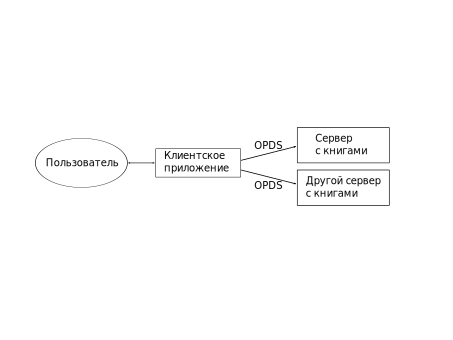
\includegraphics[width=.5\textwidth]{scheme}
%\caption{Мега-схема проекта}\label{fig:scheme}
%\end{figure}
%\picref{fig:scheme}	ссылка на картинку

\numlesschap{Заключение}

\end{document}

